\documentclass{article}
\usepackage{graphicx}
\usepackage{hyperref}
\usepackage{indentfirst}

\title{%
    Real-time Usage and Crowd Detection for Shared Facilities using Surveillance Cameras\\
  \large CS766 Proposal}
\author{Mondo Jiang, William Sun, Lao Chang}
\date{February 2024}

\begin{document}

\maketitle


\section{Introduction}
In physical scenarios with shared resources (such as restaurants, libraries, gyms, etc.), the occupancy and congestion of facilities information can provide great convenience for users and guests. Existing crowd counting algorithms mostly deal with the total number of people in a video rather than the details. However, they provide insights of how to track the overall counting though the use of machine learning (ML) algorithms and image processing techniques \cite{Chen_2020}. These methods make it possible to observe crowd dynamics in real time. 

We are interested in crowd counting through the use of CV because of the lackluster real-time occupancy report currently provided by UW-Madison's gyms. The traditional gym methods face challenges such as inability to track real-time occupancy and headcount across different areas with only manual counting, hindering resource allocation and impacting user experience\cite{bakke}. This information is crucial for users seeking to optimize their workout routines and avoid crowded areas or wait times for specific equipment.

We plan to develop a system that utilizes machine learning and traditional computer vision techniques to provide real-time occupancy statistics and headcount for different floors and specific areas within a gym, while ensuring user privacy.

\section{Related Work}
There are many approaches to CV crowd counting. Although vision-based approaches from image/video data is a very natural methodology, in a building environment such as a gym, there are many ingenious methods to accurately determine how busy each floor is.
\begin{description}
\item[Tracking with AP Points]  The use of sensors that scan for radio signals (Bluetooth and WiFi) in an area is employed in many university libraries, which can quickly and accurately assess floor occupancy \cite{waitz}. But Wi-Fi-based estimates provide only a general overview of gym occupancy without offering insights into specific areas or different types of equipment usage.
\item[Crowd Counting using Traditional Methods] Classical CV approaches to crowd counting primarily rely on using video data captured from a surveillance camera or other visual sensor. These sensors then uses various techniques to detect and count individuals. In early works, crowd counting work by detecting individual with bounding boxes. This is accurate in low density crowds. However, in overcrowded scene with severe occlusions, it is not optimal to detect every single person \cite{Zhiheng,4587569}.
\item[Convolutions Neural Networks]  More recently, convolutions neural networks (CNNs) have become popular in vision-based crowd counting. Due to the common visual features of people in a crowd, CNNs can use this prior effectively to accurately understand a scene, such as \cite{Ilyas2022,CNN}.
\end{description}

\section{Approach}


\begin{description}
\item[Data Source] For now, we will opt out of labelling data as that is too time intensive for the timeline of this course, so we will train using online datasets, and test them on both online datasets\cite{virat,https://doi.org/10.17632/xh6m6gxhvj.1} and our own captured dataset without the ground truth. For this application, it will be simple enough to visually confirm the results, so we can qualitatively analyze our custom results. 
\item[Crowd Counting] With classical CV techniques, we will re-implement the use of Gaussian mixture models to model the distribution of people within a scene. This has seen widespread success and has stood the test of time, so it is a promising approach for our application. Similarly, we are interested in comparing the classical CV techniques that we have learned in class to more modern approaches using deep learning. For this, we will look into recent architectures such as GauNet and FGENet, reimplement them, and compare them to the classical methods \cite{CNN, 9321733}.
\item[Automatic Facility Identification] To further enhance our solution, we are exploring the implementation of automatic facility identification using object detection algorithms. As an initial step, we will employ manual segmentation to divide the image frame into distinct areas representing specific facilities.
\item[Expected Result] As shown in the expected result Figure \ref{fig:expected}, we hope that the system can automatically identify the equipment and its usage status. We will also try to communicate with Bakke to try to put the system into formal use if condition permits.
\begin{figure}[ht]
    \centering
    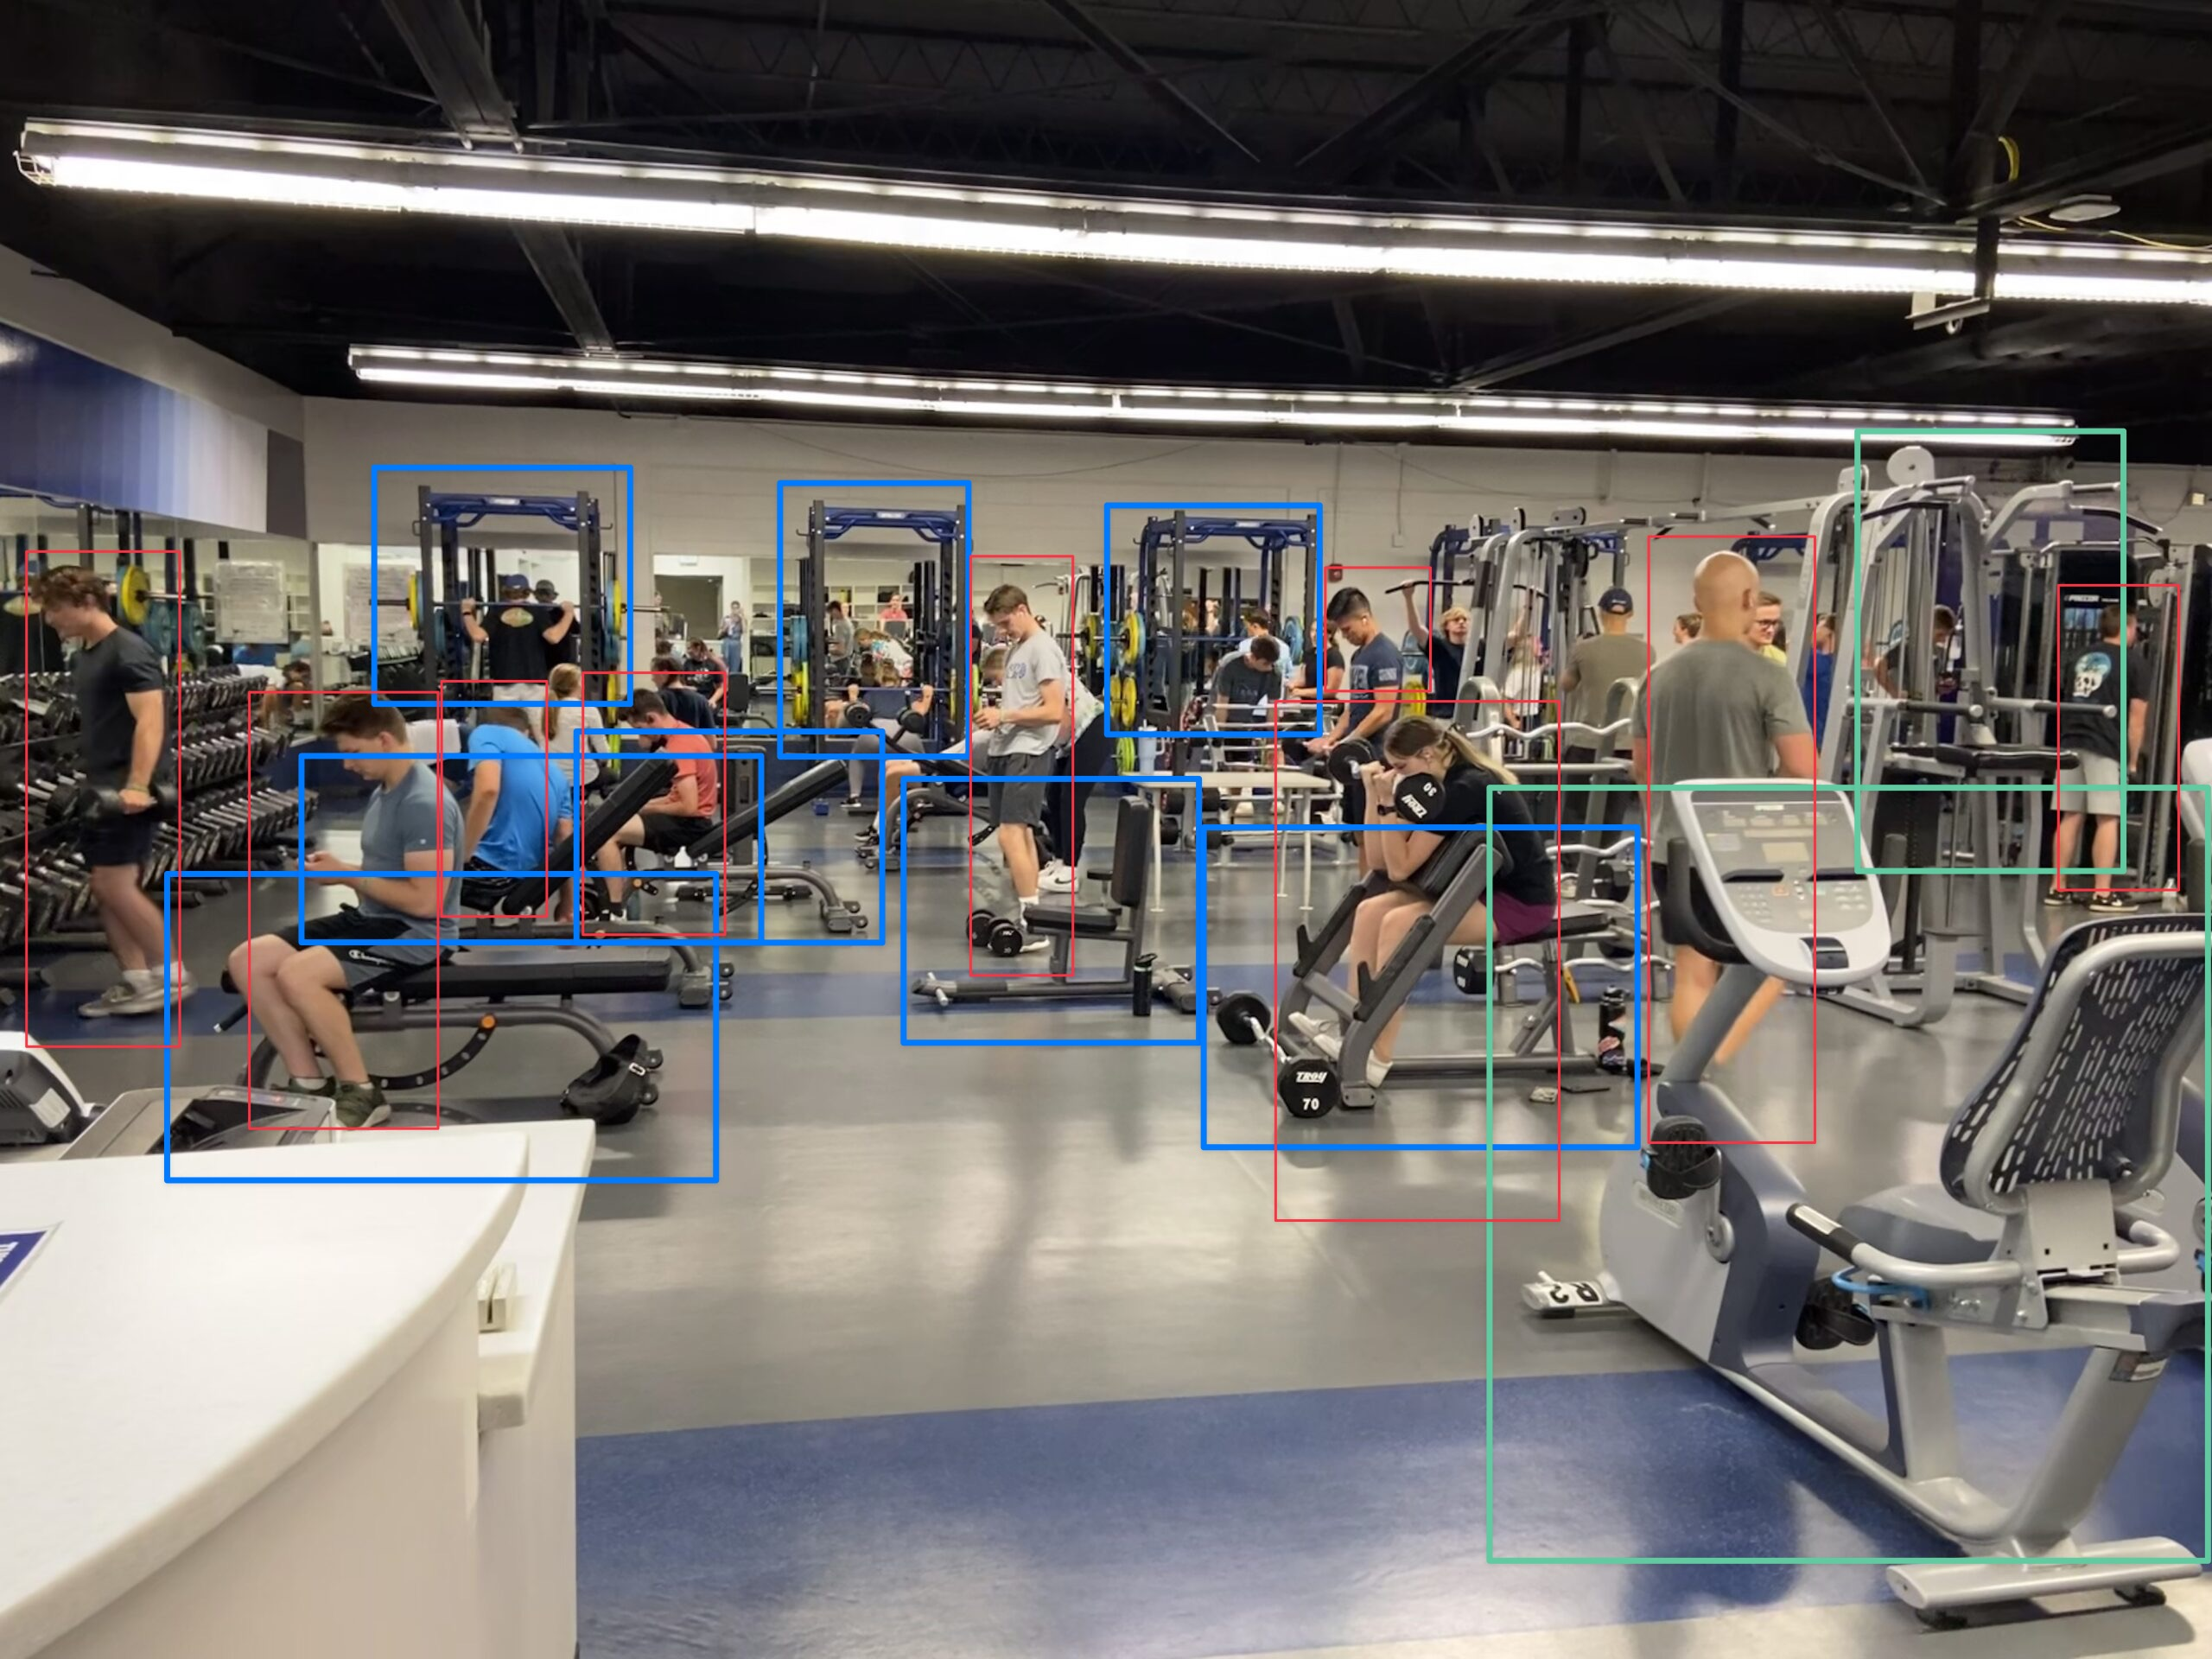
\includegraphics[width=0.8\linewidth]{expected.jpg}
    \caption{Expected result. Blue - Occupied, Green - Vacant, Red - Human}
    \label{fig:expected}
\end{figure}
\end{description}

\section{Timeline}
\begin{enumerate} % We are currently on week 5
    \item Capture custom test data (Week 6)
    \item Implement classical CV approach (Week 7), implement NN approach
    \item Implement visualizations of data/method/samples (Week 8)
    \item Midterm Report (Week 9) (Due March 22)
    % Week 10 is spring break  j
    \item Test on other datasets from the Internet (Week 11)
    \item Test on custom test data (Week 12)
    \item Week 13 will be for finishing up and miscellaneous work
    \item Presentation (Week 14 \& 15) (Due April 19), Project Webpage (Due May 3rd)
\end{enumerate}

\bibliographystyle{acm}
\bibliography{refs} % Entries are in the refs.bib file

\end{document}
